\documentclass[aspectratio=43,t,11pt]{beamer}
\usepackage{slides,math}

\title{Dynamic Treatment Effect Estimation with Interactive Fixed Effects and Short Panels}
\date{\today}
\author{Kyle Butts and Nicholas Brown}

\addbibresource{references.bib}
\begin{document}

\begin{frame}[plain]
  \maketitle

  \vspace{10mm}
  {\footnotesize
    \url{https://kylebutts.com/files/JMP.pdf}\\[-2mm]
    \url{https://kylebutts.com/files/JMP_slides.pdf}
  }
\end{frame}

\section{Motivation}

\begin{frame}{Motivation}
  Treatment is often targeted to places/units based on their economic trends:

  \begin{itemize}
    \item Place-based policies \citecolor{\citep{neumark2015place}}
    \begin{itemize}
      \item Target places with declining labor markets 
    \end{itemize}
    
    \item New apartment construction \citecolor{\citep{asquith2021local,pennington2021does}}
    \begin{itemize}
      \item Built in appreciating neighborhoods
    \end{itemize} 

    \item Walmart entry \citecolor{\citep{basker2005job,neumark2008effects}}
    \begin{itemize}
      \item Open stores in areas with growing retail spending
    \end{itemize}
  \end{itemize}

  \bigskip
  Standard difference-in-differences assumption of parallel trends is \emph{implausible}
\end{frame}

\begin{frame}{Motivation}
  In some settings, the causes of these trends are due to larger economic forces and not location-specific shocks:
  
  \begin{itemize}
    \item Place-based policies
    \begin{itemize}
      \item Decline of manufacturing hurting manufacturing hubs
    \end{itemize}
    
    \item New apartment construction
    \begin{itemize}
      \item Changing preferences for walkable neighborhoods
    \end{itemize} 

    \item Walmart entry
    \begin{itemize}
      \item Growing employment increases disposable income
    \end{itemize}
  \end{itemize}

  \bigskip
  Units have differential exposure to these macroeconomic trends in ways that are correlated with treatment
  % \purple{\textbf{Can we control for the confounding macroeconomic effects in panel settings?}}
\end{frame}

\begin{frame}{Factor Model}
  This paper models differential trends using a \textbf{factor model} generalizes the two-way fixed effect model:
  \begin{itemize}
    \item A set of macroeconomic time shocks that are common across units
    \item Units vary in how affected they are by the shocks
  \end{itemize} 
\end{frame}

\begin{frame}{This paper}
  We propose a \textbf{class of imputation-style treatment effect estimators} under a \textbf{factor model}:

  \begin{itemize}
    \item Our `imputation' style estimator explicitly estimates untreated potential outcome, $\cranberry{y_{it}(0)}$, in the post-treatment periods (similar to synthetic control)
    
    \item Treatment can be targeted based on a unit/location's exposure to shocks (violates standard parallel trends)
    
    \item Our estimator is valid in small-$T$ settings
  \end{itemize}

\end{frame}

\begin{frame}{Current approaches}{Covariates in two-way fixed effect model}\label{slide:current_approaches_cov}
  If you could observe `exposure' to some macroeconomic trend, you could include it in a two-way fixed effect model:
  $$
    \cranberry{y_{it}(0)} = \mu_i + \lambda_t + X_{i} \beta_t + u_{it}
  $$

  This allows $X_i$-specific trends, e.g. manufacturing share is given by $X_i$ and each period's `shocks' estimated by $\beta_t$
  
  \pause\smallskip
  \emph{Issues:}
  \begin{itemize}
    \item You must \emph{observe} the underlying `exposure' variables
    
    \item Noisy measures of $X_i$ only partially control for the problem \citecolor{[\citet{kejriwal2021efficacy}]} 
  \end{itemize}

  \bottomleft{\hyperlink{slide:noisy_xi_simulations}{\beamergotobutton{Simulation Evidence}}}
\end{frame}


\begin{frame}{Current approaches}{Synthetic Control} 
  The synthetic control estimator constructs a `control unit' that has the same exposure to the macroeconomic trends. 
  
  \begin{itemize}
    \item Synthetic control is consistent when $\cranberry{y_{it}(0)}$ has a factor model structure if you have a sufficiently large number of pre-periods 
  \end{itemize}

  \pause\smallskip
  \emph{Issues:}
  \begin{itemize}
    \item In short-panels, you \emph{over-fit} on noise and get bad estimates \citecolor{[\citet{abadie2010synthetic,ferman2021synthetic}]}
    
    \item Even if you have a large number of pre-periods, structural changes to the economy can make far-away pre-periods uninformative (e.g. the 2008 recession) \citecolor{[\citet{abadie2021using}]}
  \end{itemize}
\end{frame}

\begin{frame}{Contribution}{Pre-trends paper}

\end{frame}

\begin{frame}{Contribution}
  There are many estimators for treatment effects under factor models:
  \begin{enumerate}
    \item Synthetic control \citecolor{\citep{abadie2021using}}
    \item Matrix Completion \citecolor{\citep{Athey_et_al_2021}}
    \item Imputation Estimators \citecolor{\citep{Gobillon_Magnac_2016, Xu_2017}}
  \end{enumerate}

  \bigskip
  \textbf{None of these are valid in short-$T$ settings.} Our paper introduces a general method that is valid in short-$T$ settings. 

  \begin{itemize}
    \item Unlocks a large econometric literature on factor model estimation and incorporates it into causal inference methods
    \begin{itemize}
      \item e.g. use some baseline covariates $X_i$ as instruments. Need to be correlated with exposure to macroeconomic shocks
    \end{itemize}
  \end{itemize}
\end{frame}

% \begin{frame}{Contribution}
%   \citet{Callaway_Karami_2020} propose a method for treatment effect estimation with a factor model
%   \begin{itemize}
%     \item They provide a single estimator that requires a time-invariant covariate whose impact on outcomes doesn't change over time.
%     \item We instead provide a general set of estimators.
%   \end{itemize}
% 
%   \citet{freyaldenhoven2019pre} propose a method that uses some variable $x_{it}$ that is affected by the same confounder that affects $y_{it}$ but not affected by treatment.
%   \begin{itemize}
%     \item This intuition is similar to a version of our method based on common-correlated effects. 
%     \item Common-correlated effects 
%   \end{itemize}
% \end{frame}

\begin{frame}{Preview of Application}{Impact of new Walmart entry on $\log$ retail employment. TWFE estimates}
  \vspace{-7.5mm}
  \begin{figure}
    \begin{adjustbox}{width=0.9\textwidth}
      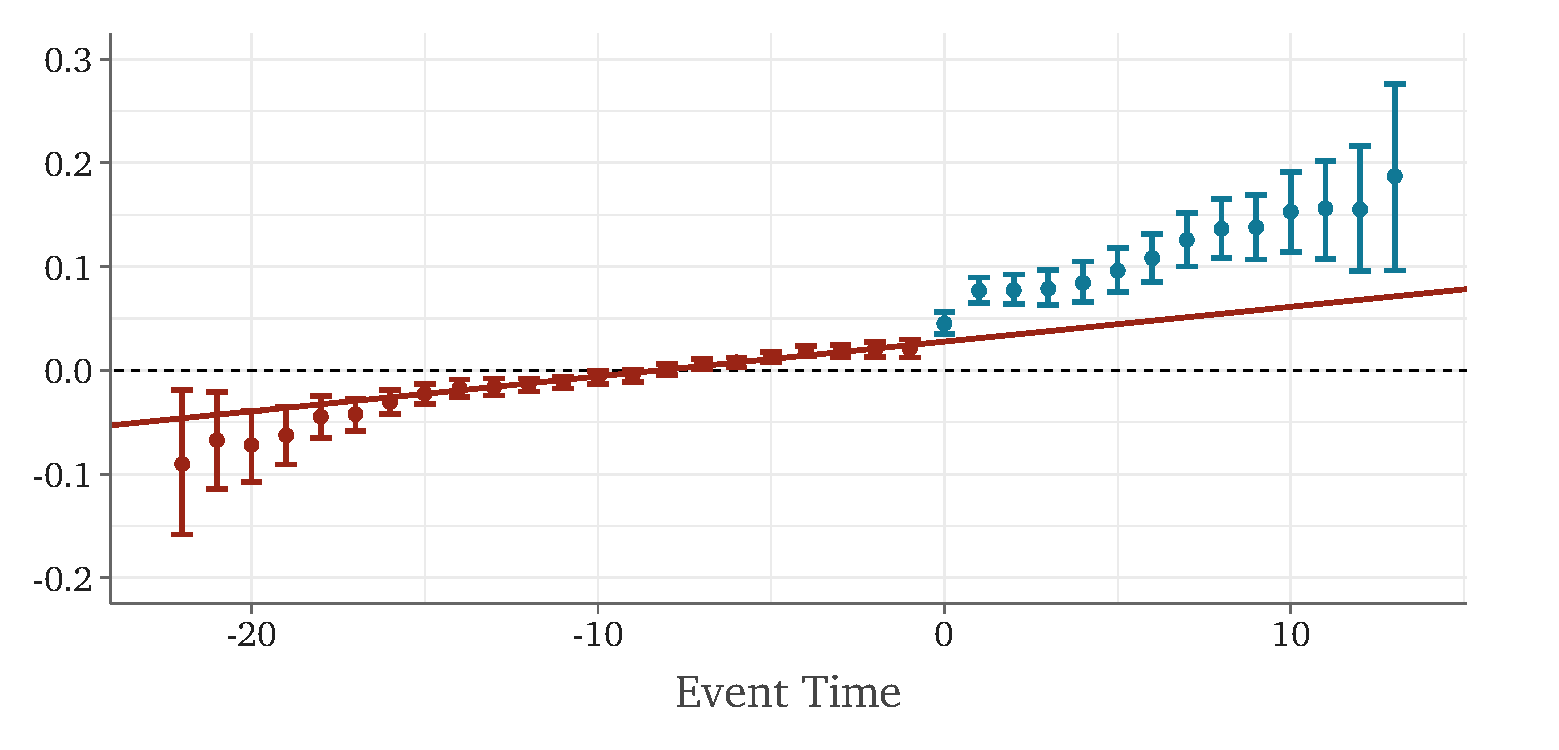
\includegraphics{../figures/plot_did2s_retail.pdf}
    \end{adjustbox}
  \end{figure}

  TWFE model expectedly is biased by non-parallel trends \citecolor{\citep{neumark2008effects,basker2005job}}
\end{frame}

\begin{frame}{Preview of Application}{Factor model estimates}
  \vspace{-7.5mm}
  \begin{figure}
    \begin{adjustbox}{width=0.9\textwidth}
      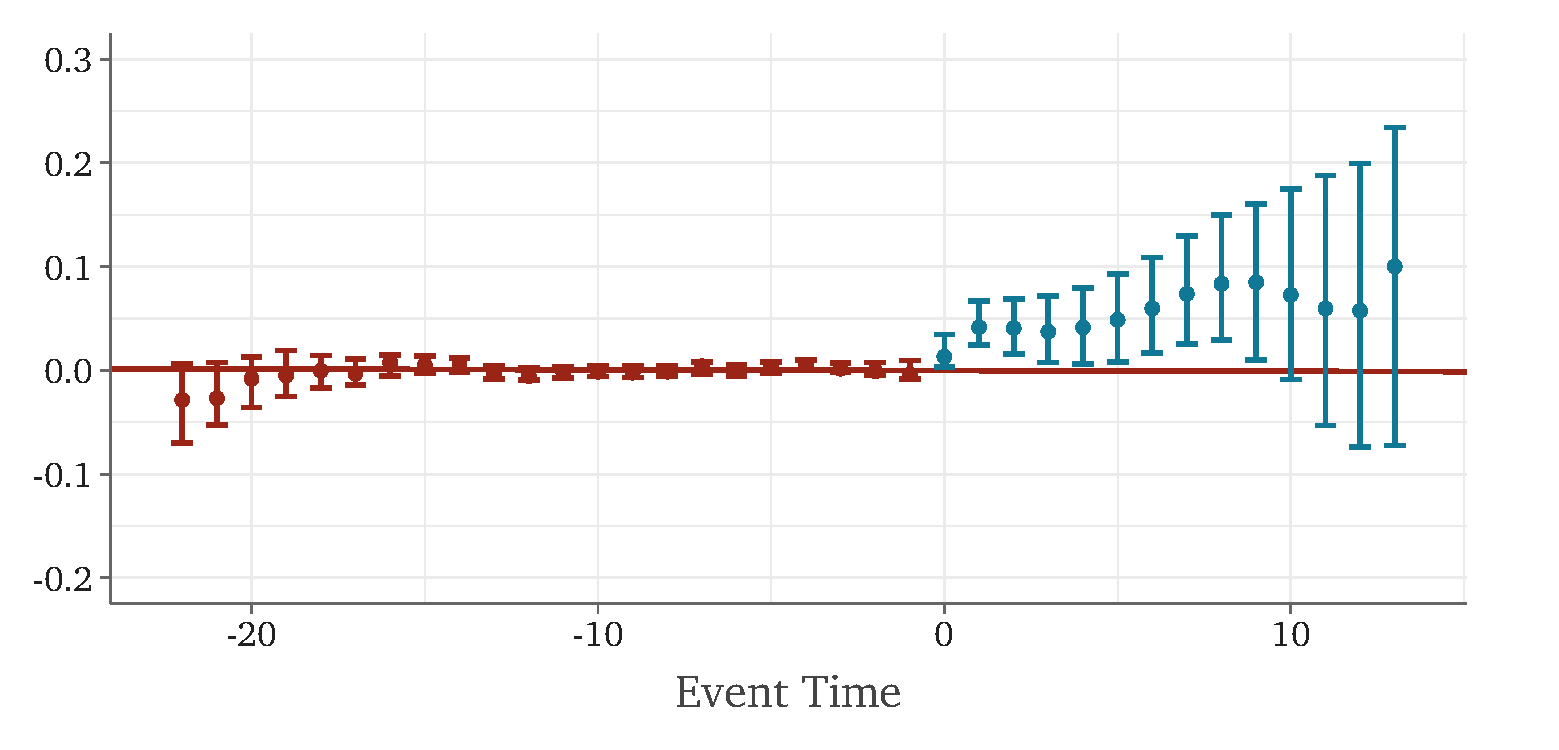
\includegraphics{../figures/plot_qld_retail.pdf}
    \end{adjustbox}
  \end{figure}

  Factor model removed systematic trend in treated outcomes
\end{frame}

% \begin{frame}{Preview of Application}{Generalized method}
%   \vspace{-7.5mm}
%   \begin{figure}
%     \begin{adjustbox}{width=0.9\textwidth}
%       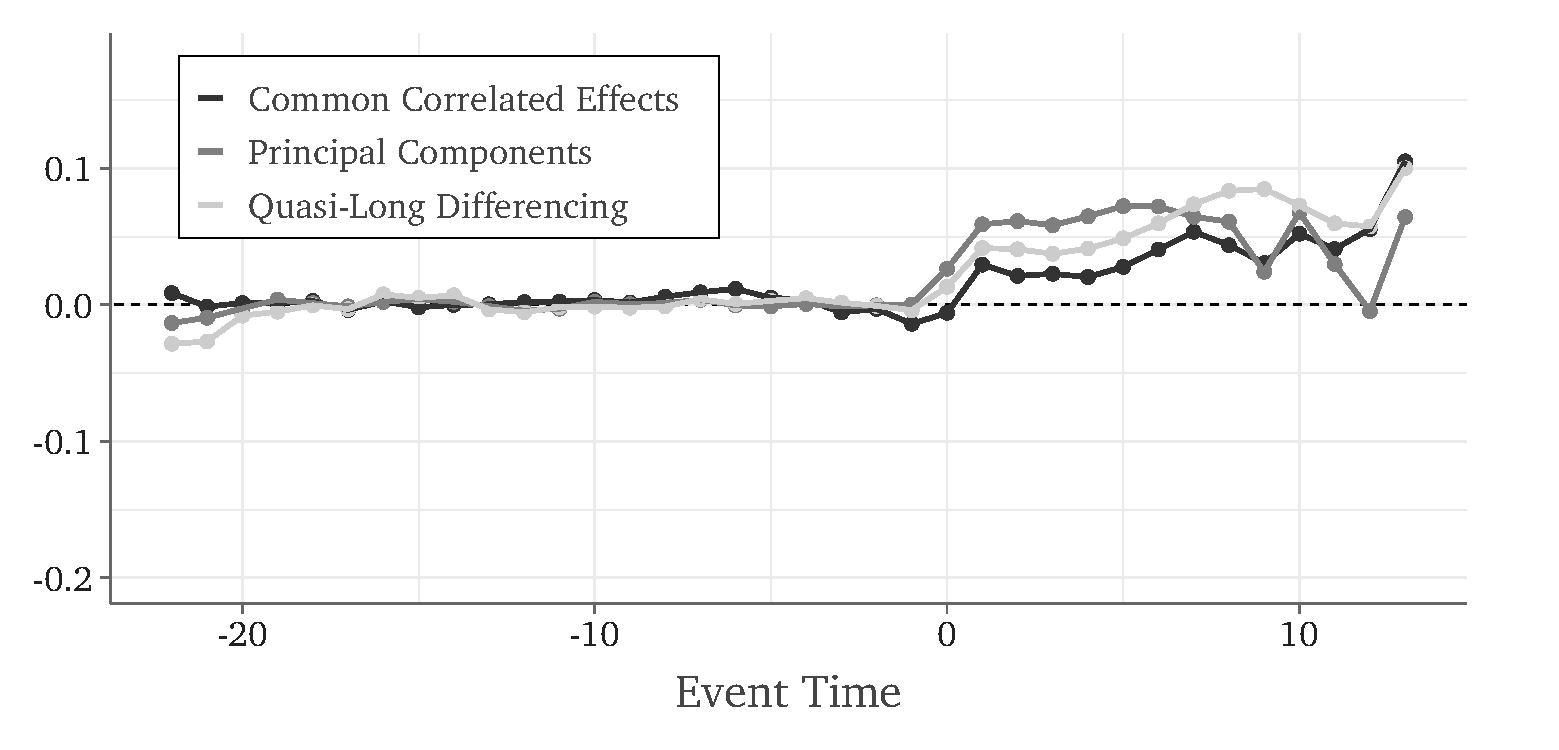
\includegraphics{../figures/plot_retail_many_estimators.pdf}
%     \end{adjustbox}
%   \end{figure}
% 
%   Our method allows many estimators for the factor shocks
% \end{frame}

% \begin{frame}{Preview of Application}{Imputation estimator}
%   \vspace{-7.5mm}
%   \begin{figure}
%     \begin{adjustbox}{width=0.9\textwidth}
%       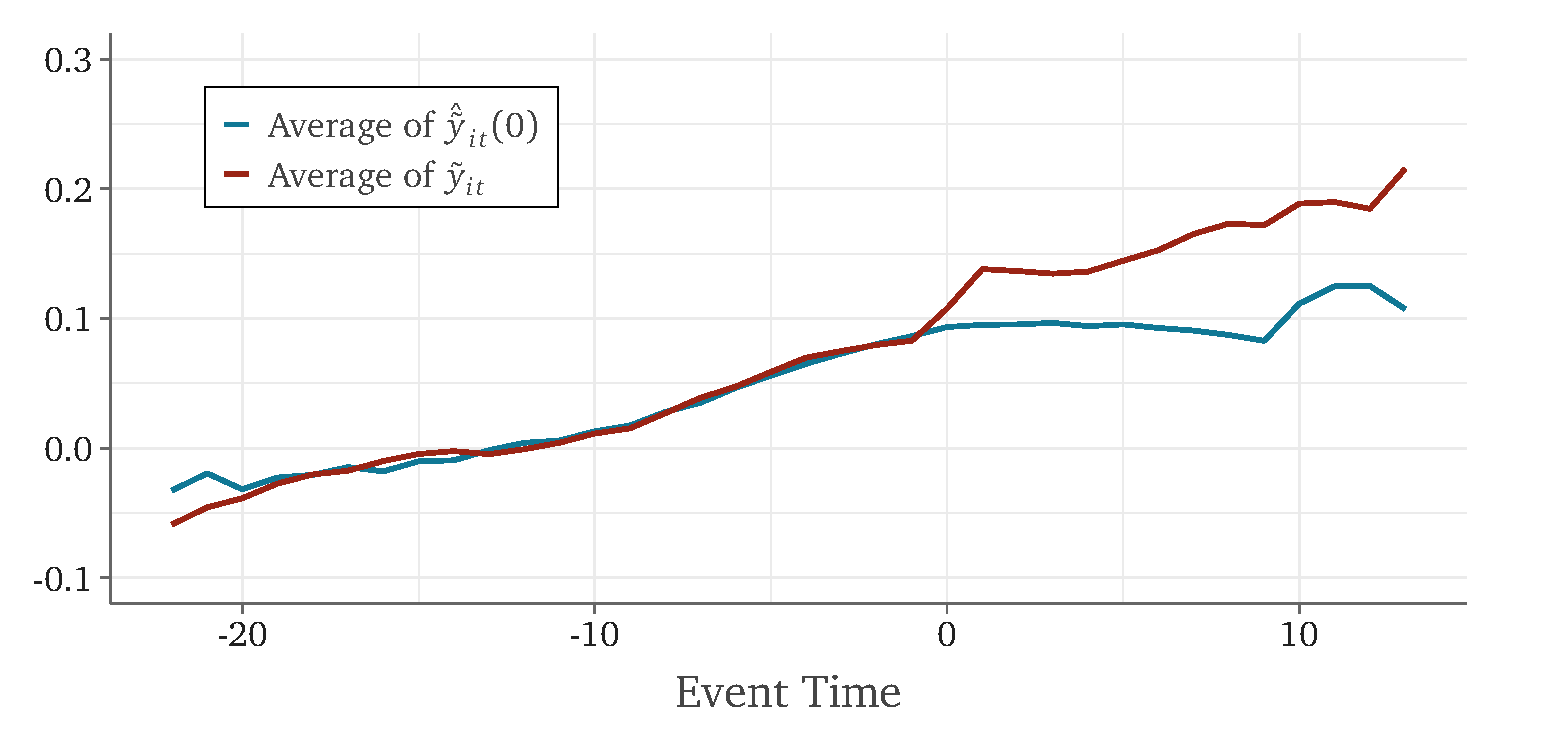
\includegraphics{../figures/plot_synth_retail.pdf}
%     \end{adjustbox}
%   \end{figure}
% 
%   Our method "imputes" $y_{it}(0)$
% \end{frame}

\section{General Identification Result}

\begin{frame}{Untreated Potential Outcomes}{Factor Model}
  We observe a panel of observations denoted by unit $i \in \{1, \dots, N\}$ and by time period $t \in \{1, \dots, T\}$. 
  
  \bigskip
  Untreated potential outcomes are given by a factor model:
  \begin{equation}\label{eq:untreated_po}
    y_{it}(0) = \sum_{r = 1}^{p} \purple{f_{t,r}} * \orange{\gamma_{i,r}} + u_{it}
  \end{equation}

  \begin{itemize}
    \item $f_{t, r}$ is the $r$-th \bgPurple{factor} (macroeconomic shock) at time $t$.
    \item $\gamma_{i,r}$ is unit i's \bgOrange{factor loading} (exposure) to the $r$-th factor.
  \end{itemize}
\end{frame}

\begin{frame}{Intuition of Factor Model}
  The intuition is very similar to that of a shift-share variable:
  $$
    z_{it} = \sum_{r = 1}^{p} f_{t,r} * \gamma_{i,r}
  $$
  \vspace*{-5mm}
  \begin{itemize}
    \item The $p \times 1$ vector $\bm{f}_t$ is the set of \emph{`macroeconomic'} shocks (shifts) that all units experience
    \item $\bm{\gamma}_i$ is an individuals \emph{exposure} (shares) to the shocks 
  \end{itemize}

  \bigskip
  The difference being that \textbf{we do not observe} the variables $\gamma_i$ and $f_t$ (like we don't observe fixed effects)
\end{frame}

\begin{frame}{Two-way Fixed Effect vs. Factor Model}
  The factor model is a generalization of the TWFE model. If $\bm{f}_{t} = (\lambda_t, 1)'$ and $\bm{\gamma}_i = (1, \mu_i)'$, then (\ref{eq:untreated_po}) becomes:
  $$
    y_{it}(0) = \lambda_t + \mu_i + u_{it}
  $$
  
  Since TWFE is the work-horse model used by applied researchers, later we will explicitly add unit and time fixed-effects back in.
\end{frame}

\begin{frame}{Treatment Effects}
  For now, assume there is a single treatment that turns on in some period $T_0 + 1$. Define $D_i$ to be a dummy to denote which units receive treatment and $d_{it}$ to equal 1 when treatment is active. 

  \pause\bigskip
  We are interested in event-study style average treatment effects. For each $t$, we define
  $$
    \text{ATT}_t \equiv \expec{y_{it}(1) - \cranberry{y_{it}(0)}}{D_i = 1},
  $$
  where $\cranberry{y_{it}(0)}$ is the (unobserved) untreated potential outcome.
\end{frame}

\begin{frame}{Assumptions}{`Non-Parallel Trends'}
  \textbf{\color{alice} Assumption:} {\color{asher} Selection into Treatment}
  $$
    \cranberry{y_{it}(0)} = \bm f_t' \bm \gamma_i + u_{it},
  $$
  where for all $t$,
  $$
    \expec{u_{it}}{\bm \gamma_i, D_i = 1} = \expec{u_{it}}{\bm \gamma_i, D_i = 0} = 0,
  $$
  
  \begin{itemize}
    \item Relaxes parallel trends by allowing units to enter treatment based on exposure to macroeconomic shocks
    
    \item Treatment can \emph{not} be correlated with unit-time specific shocks $u_{it}$ 
  \end{itemize}
\end{frame}

\begin{frame}{Assumptions}{Additional assumptions}
  \textbf{\color{alice} Assumption:} {\color{asher} Arbitrary Treatment Effects}
  \begin{equation}
    y_{it}(1) = \cranberry{y_{it}(0)} + \tau_{it}
  \end{equation}

  \bigskip
  \textbf{\color{alice} Assumption:} {\color{asher} No Anticipation}
  $$
    \cranberry{y_{it}(0)} = y_{it} \text{ when } d_{it} = 0
  $$
\end{frame}

% \begin{frame}{Selection into Treatment and Parallel Trends}
%   In the two period case ($t = 1, 0$) consider the difference-in-differences estimand with parallel trends on the error term:
%   \begin{align*}
%       & \mathbb{E}_{i} \left[ y_{i1}(1) - y_{i0}(0) \ \vert \ D_i = 1 \right] - \mathbb{E}_{i} \left[ y_{i1}(1) - y_{i0}(0) \ \vert \ D_i = 0 \right] \\ 
%       \only<2> {
%         &= \mathbb{E}_{i} \left[ \tau_{i1} \ \vert \ D_i = 1 \right] + \bm f_t' \big( \mathbb{E}_{i} \left[ \bm{\gamma}_i \ \vert \ D_i = 1 \right] - \mathbb{E}_{i} \left[ \bm{\gamma}_i \ \vert \ D_i = 0 \right] \big)
%       }
%   \end{align*}
% 
%   \bigskip
%   \only<2>{This last term makes parallel trends not hold. That is, differential exposure to macroeconomic shocks violates parallel trends!}
% \end{frame}

\begin{frame}{$\text{ATT}_t$ Identification}
  For a given $t$, the average outcome for the treated sample:
  \begin{align*}
    \text{ATT}_t &\equiv \mathbb{E}_{i} \left[ y_{it}(1) \ \vert \ D_i = 1 \right] - \mathbb{E}_{i} \left[ \cranberry{y_{it}(0)} \ \vert \ D_i = 1 \right] \\
    &= \mathbb{E}_{i} \left[ y_{it}(1) \ \vert \ D_i = 1 \right] - \bm{f}_t' \mathbb{E}_{i} \left[ \bm{\gamma}_i \ \vert \ D_i = 1 \right],
  \end{align*}
  where the equality comes from our selection into treatment assumption.  

  \bigskip
  \textbf{Insight:} Estimating each $\bm{\gamma}_i$ requires large-$T$
  \begin{itemize}
    \item We only need to estimate $\left[ \bm{\gamma}_i \ \vert \ D_i = 1 \right]$ which is possible in small-$T$ settings
  \end{itemize}
\end{frame}

\begin{frame}{$\text{ATT}_t$ Identification}
  Suppose we observed the $T \times p$ matrix of factors, $\bm{F}$. Let `$\text{pre}$' denote the time periods before treatment $t \leq T_0$. 
  
  \bigskip
  Then for $t > T_0$,
  \begin{align*}
    &\mathbb{E}_i \big[%
      y_{it} - \bm{f}_t' (\bm{F}_{\text{pre}}' \bm{F}_{\text{pre}})^{-1} \bm{F}_{\text{pre}}'
      \underbrace{\bm y_{i, \text{pre} } }_{\bm{F}_{\text{pre}} \bm{\gamma}_i + \bm{u}_{i,\text{pre}}} \ \vert \ D_i = 1
    \big]
    \\
    &\quad = \expec[i]{y_{it} - \bm{f}_t' \bm{\gamma}_i}{D_i = 1} 
    \\
    &\quad = \expec[i]{y_{it} - \cranberry{y_{it}(0)}}{D_i = 1}
    \\ 
    &\quad = ATT_t
  \end{align*}
\end{frame}

\begin{frame}{$ATT_t$ Identification}{General Procedure}\label{slide:general_imputation_procedure}
  \vspace{-7.5mm}
  $$
    ATT_t = \expec[i]{%
      y_{it} - \bm{f}_t' (\bm{F}_{\text{pre}}' \bm{F}_{\text{pre}})^{-1} \bm{F}_{\text{pre}}' \bm y_{i, \text{pre} } 
    }{D_i = 1} 
  $$

  Consistency possible with $\sqrt{n}$-consistent estimation of the factors $\bm{F}$. \hyperlink{slide:column_space_condition}{\beamergotobutton{Requirements for factor estimates, $\hat{\bm{F}}$}}

  \begin{itemize}
    \item This brings in a large literature on factor model estimation to causal-inference methods
    \begin{itemize}
      \item Will illustrate multiple estimators of $\bm{F}$ in application. 
    \end{itemize}
    
    \pause \item Use only untreated observations, $d_{it} = 0$, for estimation of $\bm{F}$ to avoid bias.
    \item Staggered treatment `imputes' $y_{it}(0)$ seperately for each treatment-timing group (changing $\text{pre}$)
  \end{itemize}
\end{frame}

\begin{frame}{Removing additive effects}\label{slide:remove_additive_fe}
  Now, we extend our base model to include additive effects
  $$
    y_{it} = \mu_i + \lambda_t + \sum_{r = 1}^{p} f_{t,r} * \gamma_{i,r} + u_{it}
  $$
  
  We within-transform the outcome to remove the fixed effects:
  $$
    \tilde{y}_{it} = y_{it} - \overline{y}_{0,t} - \overline{y}_{i,pre} + \overline{y}_{0,pre}
  $$

  \begin{itemize}
    \item $\overline{y}_{0,t}$: never-treated cross-sectional averages.
    \item $\overline{y}_{i,pre}$: pre-treated time averages.
    \item $\overline{y}_{0,pre}$: overall never-treated pre-treated average.
  \end{itemize}

  \hyperlink{slide:twfe_test}{\beamergotobutton{Test for TWFE Model Sufficiency}}
\end{frame}

\begin{frame}{Removing additive effects}
  \vspace{-\bigskipamount}
  $$
    \tilde{y}_{it} = y_{it} - \overline{y}_{0,t} - \overline{y}_{i,pre} + \overline{y}_{0,pre}
  $$

  \bigskip
  After performing our transformation, we have:
  $$
    \expec{\tilde{y}_{it}}{D_i = 1} = \expec{d_{it} \tau_{it} + \tilde{\bm f}_t' \tilde{\bm \gamma}_i }{D_i = 1}
  $$
  where $\tilde{\bm f}_t$ are the pre-treatment demeaned factors and $\tilde{\bm \gamma}_i$ are the never-treated demeaned loadings.

  \begin{itemize}
    \item \textbf{Novel result:} Our transformation removes $(\mu_i, \lambda_t)$ but preserves a common factor structure $\implies$ our imputation argument holds on transformed outcomes.
  \end{itemize}
\end{frame}

\section{Example Estimators and Empirical Application}

\begin{frame}{Empirical Setting}
  We reevaluate the affect of Walmart openings on local labor markets. Mixed results in empirical literature \citecolor{[\citet{basker2005job,neumark2008effects,basker2007good,volpe2022economic}]}.

  \pause\bigskip
  Walmart opens stores based on local economic trajectories.
  \begin{itemize}
    \item Plausibly, Walmart is not targeting a specific location based on local shocks, i.e. based on $u_{it}$.

    \item Identification is based on assumption that Walmart picks places with growing retail sector due to national economic conditions, i.e. based on $\bm{f}_t \bm{\gamma}_i$.
  \end{itemize}
\end{frame}

\begin{frame}{Data}
  We construct a dataset following the description in \citet{basker2005job}.

  \begin{itemize}
    \item In particular, we use the County Business Patterns dataset from 1964 and 1977-1999
    \item Subset to counties that (i) had more than 1500 employees overall in 1964 and (ii) had non-negative aggregate employment growth between 1964 and 1977
  \end{itemize}

  \smallskip\pause
  We use a geocoded dataset of Walmart openings from \citet{arcidiacono2020competitive}

  \begin{itemize}
    \item Treatment dummy is equal to one if the county has any Walmart in that year and our group variable denotes the year of entrance for the \emph{first} Walmart in the county.
  \end{itemize}
\end{frame}

\begin{frame}{Initial Estimates}
  To show problems with selection, we estimate a TWFE imputation model \citecolor{[\citet{Wooldridge_2021,Borusyak_Jaravel_Spiess_2021}]}:
  \begin{equation}
      \log(y_{it}) = \mu_i + \lambda_t + \sum_{\ell = -22}^{13} \tau^\ell d_{it}^\ell + e_{it},
  \end{equation}
  \begin{itemize}
    \item $y_{it}$ include county-level retail employment and wholesale employment.
    \item $d_{it}^\ell$ are event-time dummies for being $\ell$ years away from when the initial Walmart opens in a county.
  \end{itemize}
\end{frame}

\begin{frame}
  \begin{figure}
    \caption{Effect of Walmart on County $\log$ Retail Employment (TWFE Estimate)}
    \begin{adjustbox}{width=\textwidth}
      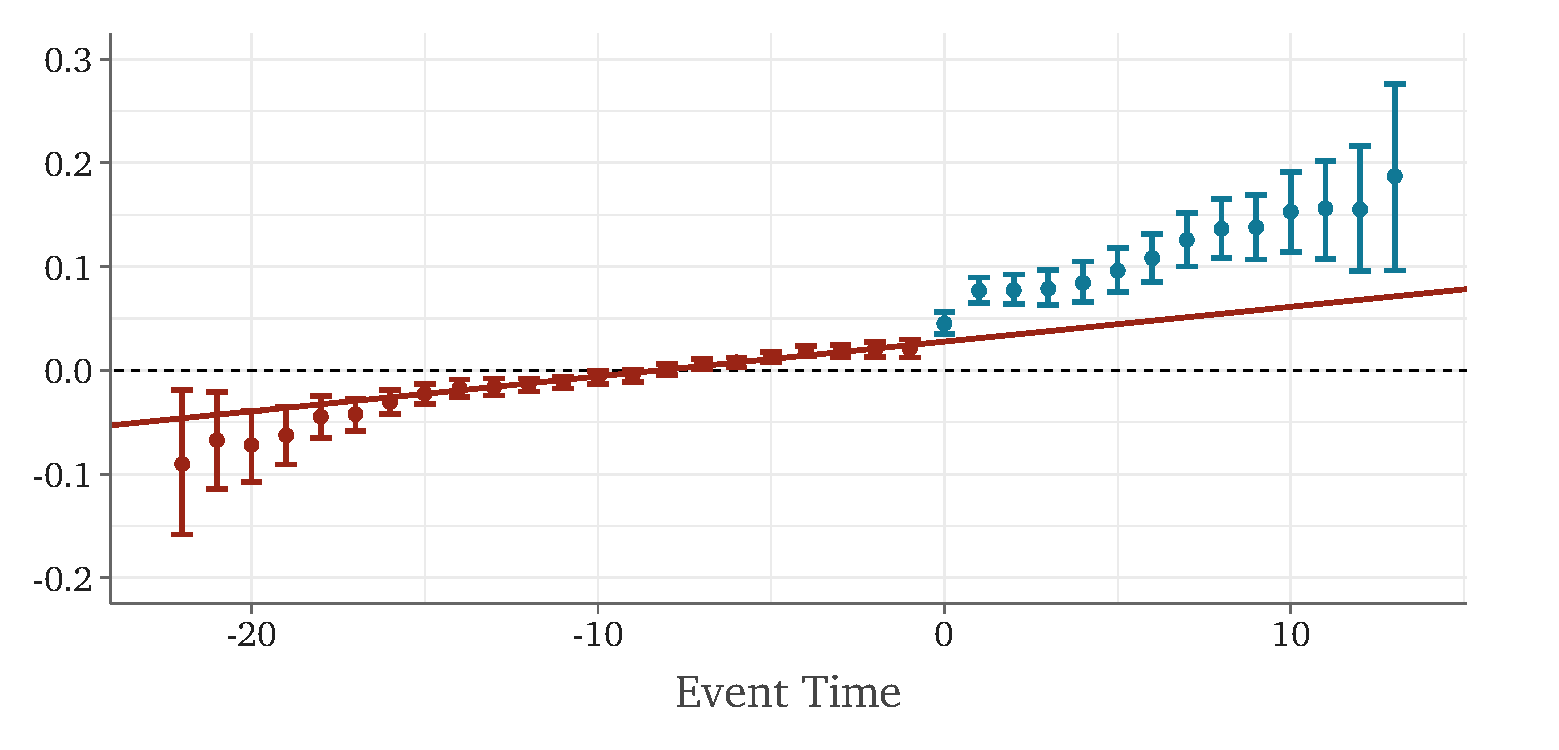
\includegraphics{../figures/plot_did2s_retail.pdf}
    \end{adjustbox}
  \end{figure}
\end{frame}

\begin{frame}
  \begin{figure}
    \caption{Effect of Walmart on County $\log$ Wholesale Employment (TWFE Estimate)}
    \begin{adjustbox}{width=\textwidth}
      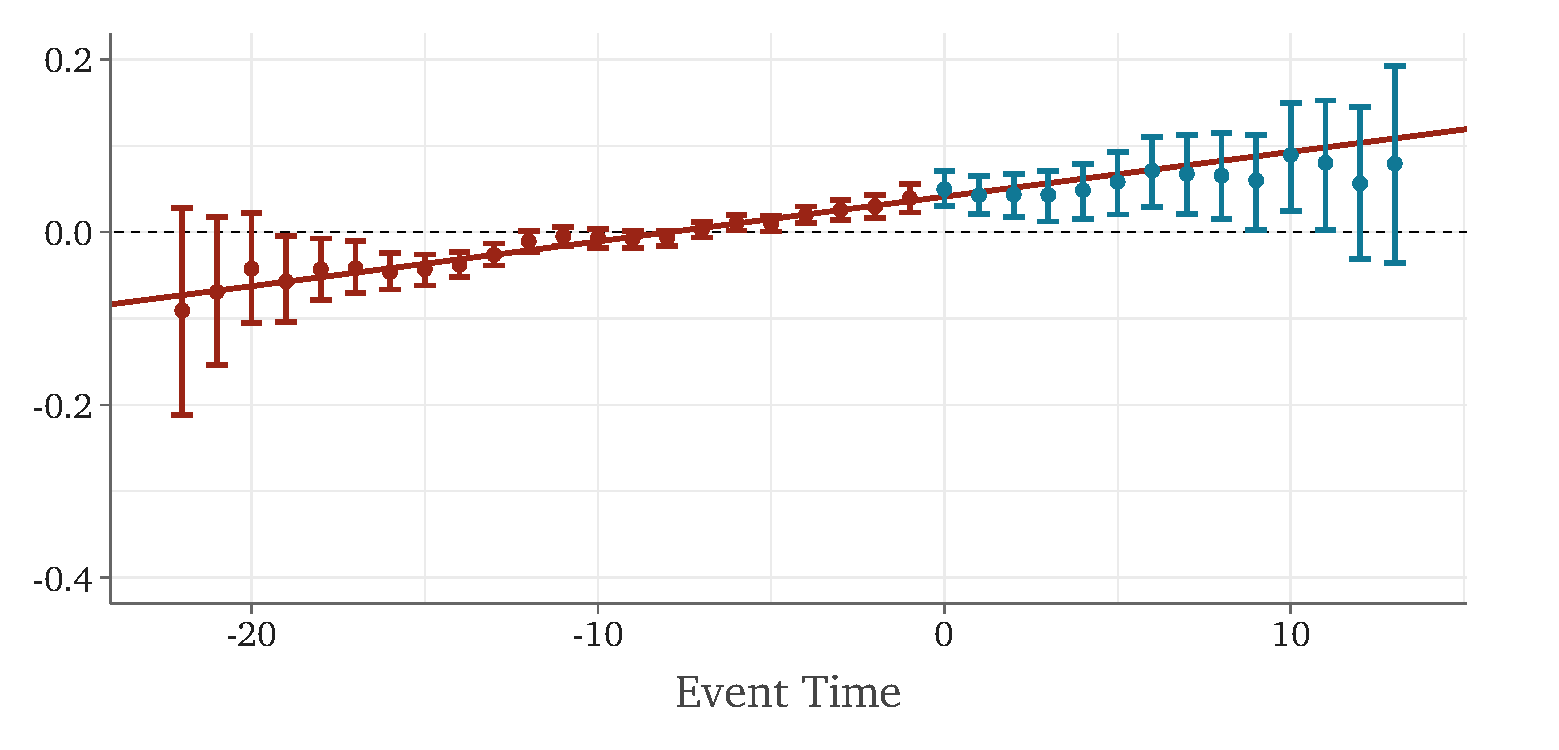
\includegraphics{../figures/plot_did2s_wholesale.pdf}
    \end{adjustbox}
  \end{figure}
\end{frame}

\begin{frame}{Factor Identification}{Strategy 1: IV strategy}\label{slide:qld_strategy}
  We consider instrumental-variables based identification strategy as proposed in \citet{Ahn_Lee_Schmidt_2013}.
  \begin{itemize}
    \item Allows fixed-$T$ identification of $\bm{F}$.
    \item A GMM estimator $\implies$ inference is standard
  \end{itemize}

  \bottomleft{\hyperlink{slide:qld_details}{\beamergotobutton{Quasi-long Differencing Details}}}
\end{frame}

\begin{frame}{Factor Identification}{Strategy 1: IV strategy}
  Intuitively, we need a set of instruments that we think:

  \begin{itemize}
    \item {\color{zinc500} (Relevancy)} Are correlated with the factor-loadings $\gamma_i$.

    \item {\color{zinc500} (Exclusion)} Satisfy an exclusion restriction on $u_{it}$. We can't pick up on $(i,t)$ shocks that are correlated with treatment
  \end{itemize}

  \bigskip
  We think the best IV strategy entails using time-invariant characteristics $X_i$ that we think are correlated with $\gamma_i$ as instruments
\end{frame}

\begin{frame}{Factor Model}
  Turning to our factor model estimator, we use the following variables at their 1980 baseline values as instruments:
  \begin{itemize}
    \item share of population employed in manufacturing
    \item shares of population below and above the poverty line
    \item shares of population employed in the private-sector and by the government
    \item shares of population with high-school and college degrees
  \end{itemize}

  \smallskip\pause
  Think that these are predictive of the kinds of economic trends Walmart may be targeting
  \begin{itemize}
    \item Using baseline values helps us avoid picking up on concurrent shocks that are correlated with walmart opening
  \end{itemize}
\end{frame}

\begin{frame}{}
  \vspace{-\bigskipamount}
  \begin{figure}
    \caption{Effect of Walmart on County $\log$ Retail Employment (Factor Model)}
    \begin{adjustbox}{width=\textwidth}
      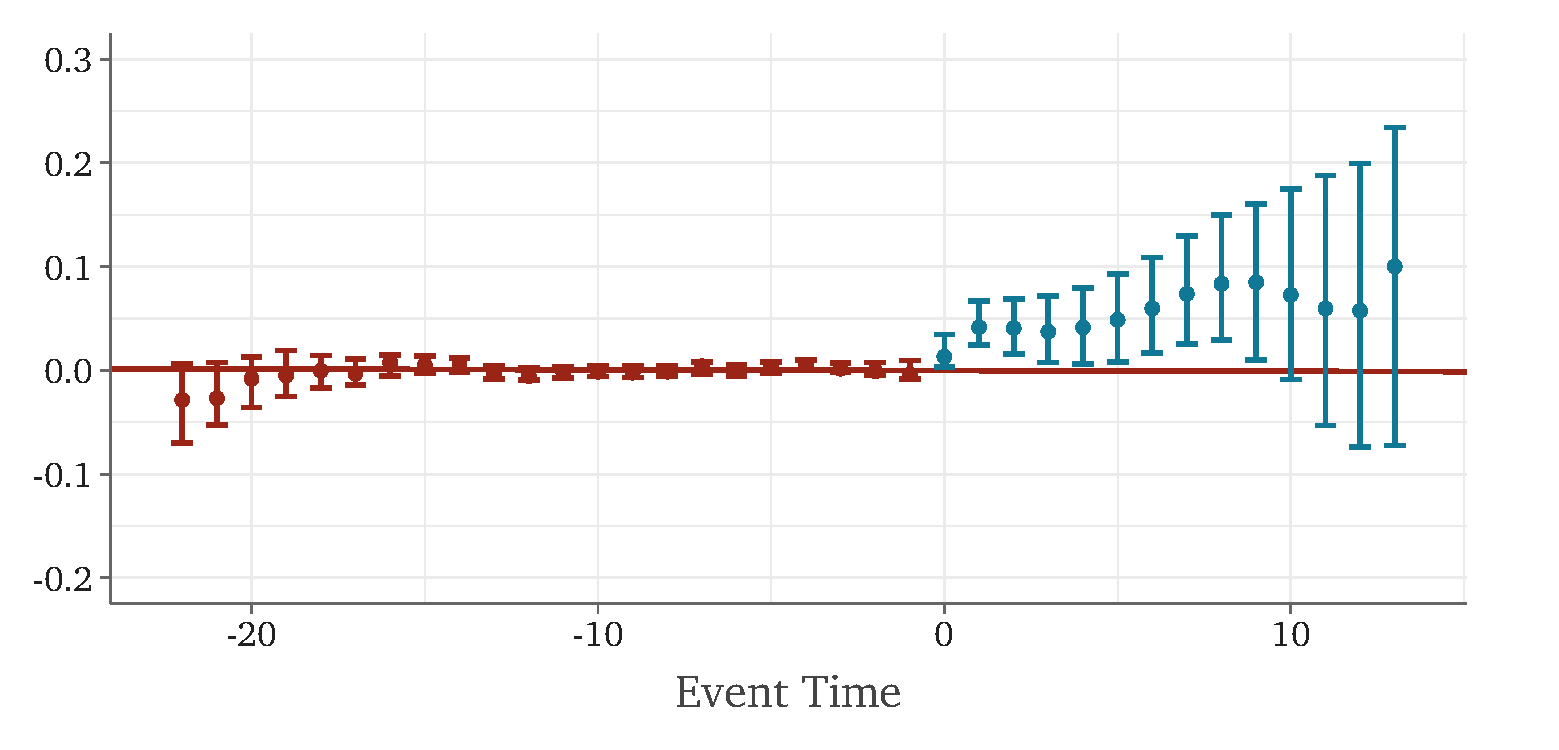
\includegraphics{../figures/plot_qld_retail.pdf}
    \end{adjustbox}
  \end{figure}

  Increase of retail employment of around 5\%, consistent with estimates in \citet{basker2005job}
\end{frame}


\begin{frame}{}
  \vspace{-\bigskipamount}
  \begin{figure}
    \caption{Effect of Walmart on County $\log$ Wholesale Employment (Factor Model)}
    \begin{adjustbox}{width=\textwidth}
      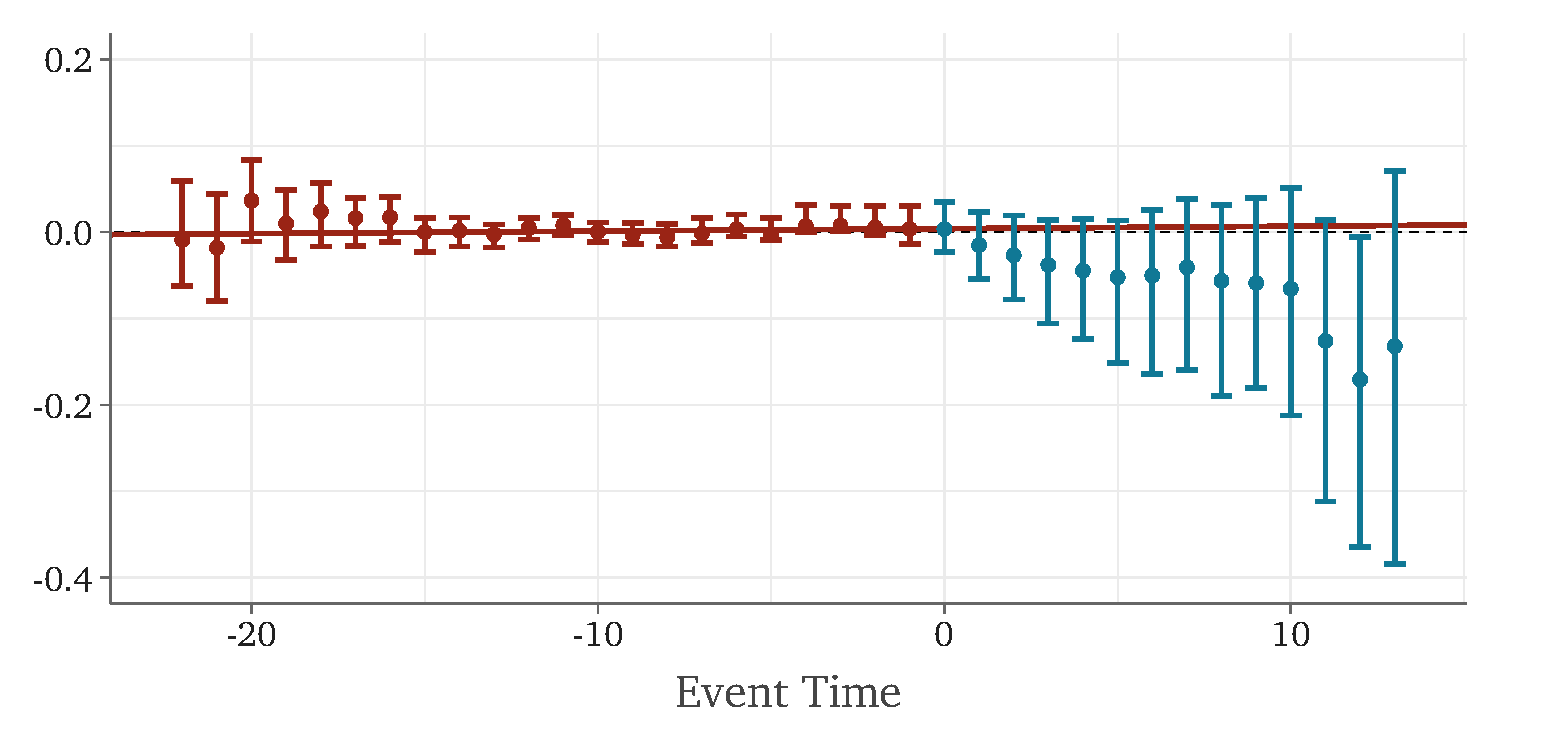
\includegraphics{../figures/plot_qld_wholesale.pdf}
    \end{adjustbox}
  \end{figure}

  Consistent with estimates in \citet{basker2005job}.
\end{frame}

\begin{frame}{Alternative identification strategies}{Strategy 2: Principal Components}
  An alternative identification strategy is a principal component decomposition of outcomes. 
  \begin{itemize}
    \item This method requires no additional variables
    \item Requires either a large number of pre-periods \citecolor{[\citet{Xu_2017}]} or error term $u_{it}$ to be uncorrelated \citecolor{[\citet{Imbens_Kallus_Mao_2021}]}
  \end{itemize} 

  \bottomleft{
    \hyperlink{slide:pc_details}{\beamergotobutton{Principal Components Details}}
  }
\end{frame}

\begin{frame}{Alternative identification strategies}{Strategy 3: Common Correlated Effects}
  The common correlated effects estimate is based on the availability of a set of additional covariates $\bm{x}_{it}$ that are affected by the same factors as $y_{it}$ \citecolor{[\citet{pesaran2006estimation}]}
  
  \begin{itemize}
    \item Cross-sectional averages of $\bm{x}_{it}$ across never-treated $i$ become proxies $\hat{\bm{F}}_t$. Need $\geq p$ covariates.
  \end{itemize}

  \bigskip
  In our Walmart setting, we use the log employment for the manufacturing, construction, agriculture, and healthcare 2-digit NAICS codes for $\bm{x}_{it}$

  \bottomleft{
    \hyperlink{slide:cce_details}{\beamergotobutton{Common Correlated Effects Details}}
  }
\end{frame}

\begin{frame}{}
  \vspace{-\bigskipamount}
  \begin{figure}
    \caption{Effect of Walmart on County $\log$ Retail Employment (Factor Model)}
    \begin{adjustbox}{width=\textwidth}
      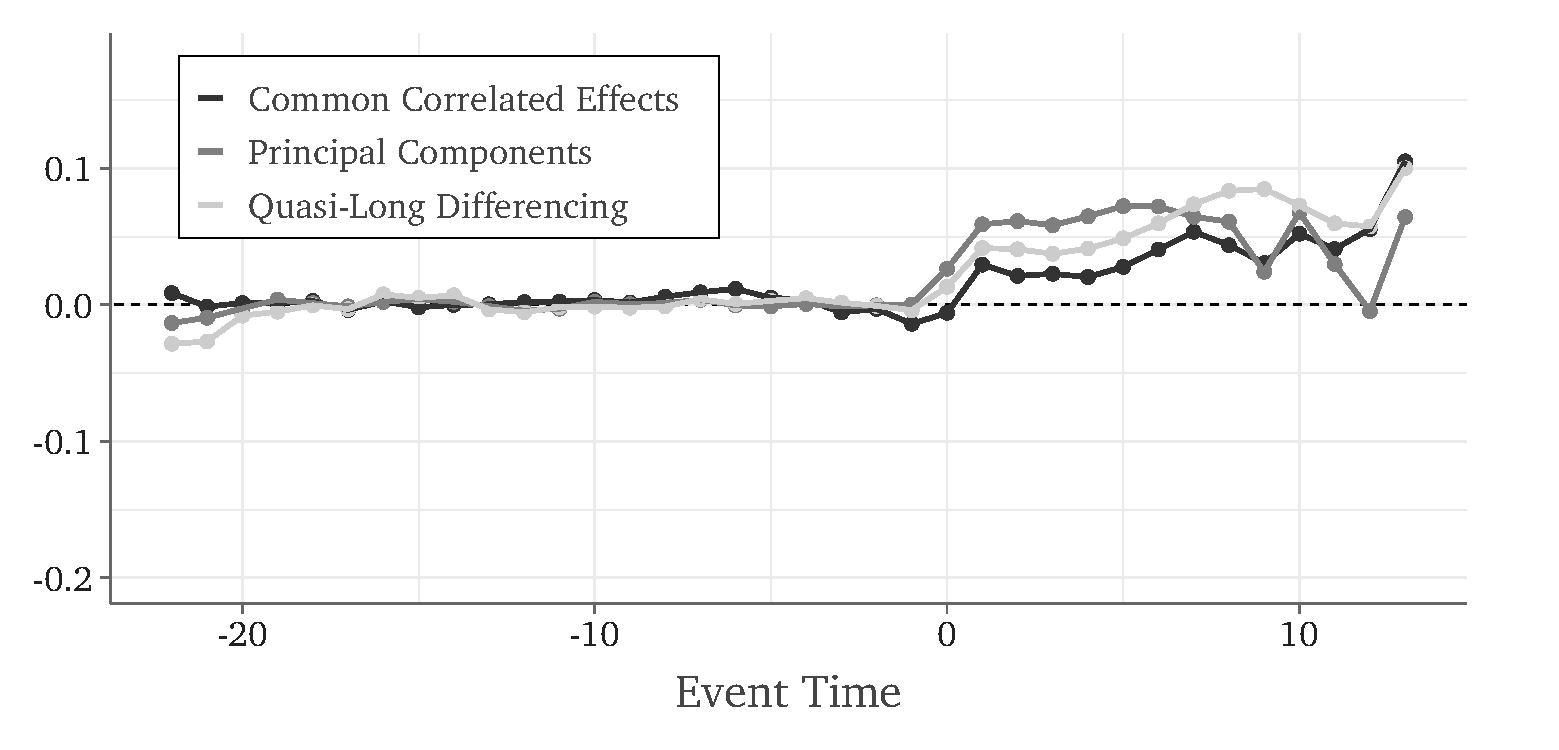
\includegraphics{../figures/plot_retail_many_estimators.pdf}
    \end{adjustbox}
  \end{figure}

  Consistent with estimates in \citet{basker2005job}.
\end{frame}

\begin{frame}{Conclusion}
  \begin{itemize}
    \item Present a fixed-T imputation procedure to identify treatment effects under a factor-model 
    
    \item Allows for differential trends between treated and control groups based on differential exposure to macroeconomic trends
    
    \item Proposed instrument-based identification of factors by using baseline characteristics that correlate with the factor-loadings
  \end{itemize}
\end{frame}

% ------------------------------------------------------------------------------
\begin{frame}[allowframebreaks]{References}
  \printbibliography
\end{frame}
\appendix
% ------------------------------------------------------------------------------

\begin{frame}{Removing additive effects}
  We consider the residuals after within-transforming
  $$
    \tilde{y}_{it} = y_{it} - \overline{y}_{0,t} - \overline{y}_{i,pre} + \overline{y}_{0,pre},
  $$
  \begin{gather*}
    \overline{y}_{i, pre} = \frac{1}{T_0} \sum_{t = 1}^{T_0} y_{it} \\
    \overline{y}_{0, t} = \frac{1}{N_{0}} \sum_{i = 1}^N (1 - D_i) y_{it} \\
    \overline{y}_{0, pre} = \frac{1}{T_0} \sum_{t = 1}^{T_0} y_{0, t}
  \end{gather*}

  % \bottomleft{ 
  %   \hyperlink{Back}{\beamergotobutton{back-within_transformation}}
  % }
\end{frame}

\begin{frame}{}\label{slide:noisy_xi_simulations}
  \begin{figure}
    \caption{TWFE model with noisy proxy variable $w_i = X_i + v_i$}
    \begin{adjustbox}{width=\textwidth}
      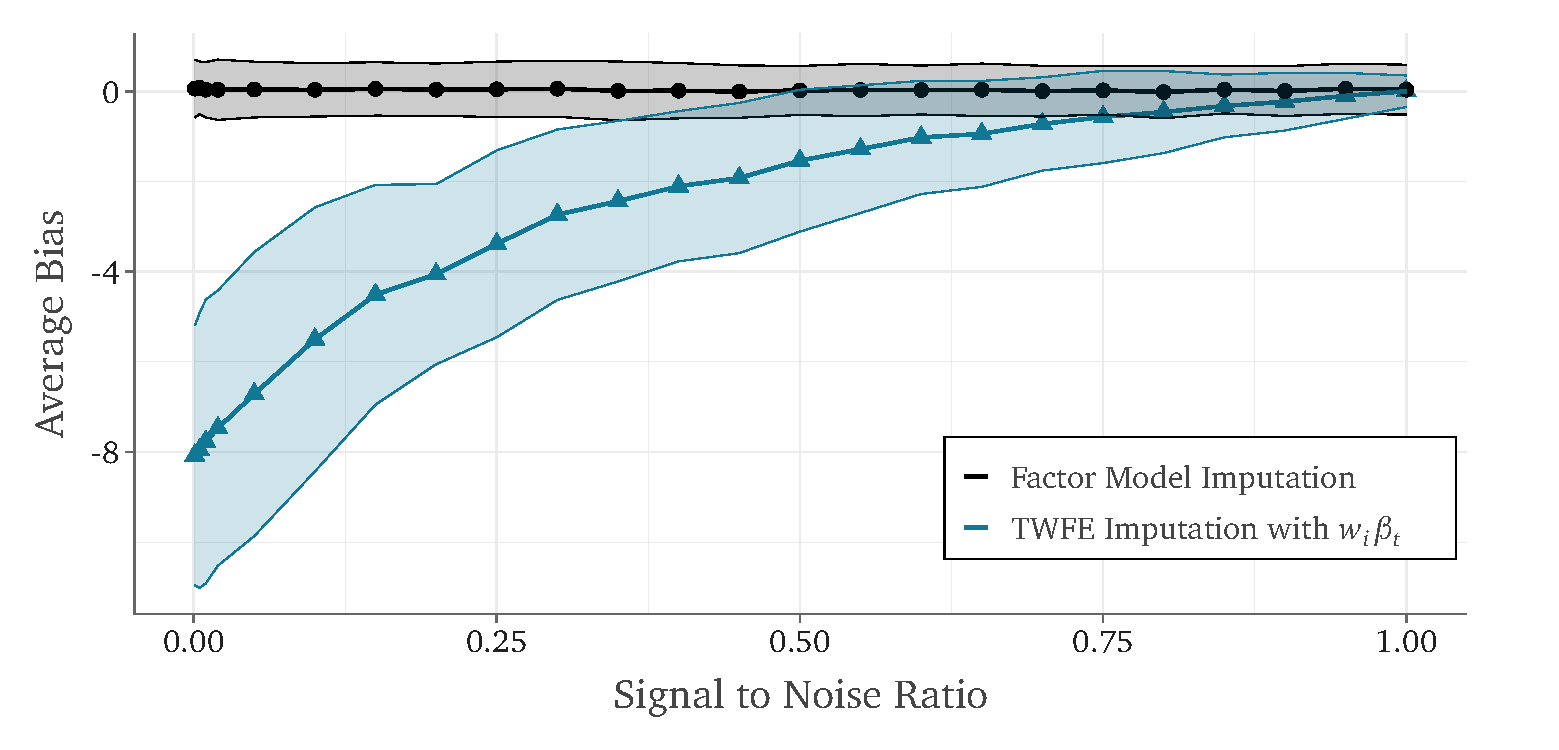
\includegraphics{../figures/simulation-bias_signal_to_noise.pdf}
    \end{adjustbox}
  \end{figure}

  \bottomleft{
    \hyperlink{slide:current_approaches_cov}{\beamergotobutton{Back}}
  }
\end{frame}


\begin{frame}{Test for TWFE Model}\label{slide:twfe_test}
  If $\expec{\bm \gamma_i}{D_i} = \expec{\bm \gamma_i}$, the ATTs are identified by the modified TWFE transformation.

  \begin{equation}\label{eq:twfe_loading_equality}
    \expec{\tilde{y}_{it}}{D_i = 1} = \expec{\tau_{it}}{D_i = 1} = \tau_t
  \end{equation}
  for $t > T_0$.

  \pause
  \begin{itemize}
    \item Says TWFE is sufficient even if there are factors, so long as exposure to these factors are the same between treated and control group.
  \end{itemize}
  
  \medskip
  In the paper, we provide tests for (\ref{eq:twfe_loading_equality})

  \bottomleft{
    \hyperlink{slide:remove_additive_fe}{\beamergotobutton{Back}}  
  }
\end{frame}

\begin{frame}{Factor Identification}\label{slide:column_span_condition}
  We cannot identify $\bm F$ or $\bm \gamma_i$ seperately from one another. 
  \begin{itemize}
    \item Rotation problem means we can only identify $A \bm F$ for some matrix $A$.
  \end{itemize}

  Consider some estimator $\bm{F}(\theta)$ such that the true factor matrix $\bm{F} \in \text{col}(\bm{F}(\theta))$
  \begin{itemize}
    \item \textbf{Examples:} common correlated effects, principal components, quasi-differencing.
  \end{itemize}

  \smallskip
  Then using $\bm{F}(\theta)$ in place of $\bm{F}$ still identifies $\text{ATT}_t$.
  \begin{itemize}
    \item $\bm{f}_t (\bm{F}_{\text{pre}}' \bm{F}_{\text{pre}})^{-1} \bm{F}_{\text{pre}}$ is invariant to rotating by any matrix $A$.
  \end{itemize}

  \bottomleft{\hyperlink{slide:general_imputation_procedure}{\beamergotobutton{Back}}}
\end{frame}


\begin{frame}{Quasi-long Differencing Details}\label{slide:qld_details}
  The quasi-long differencing method \citecolor{\citet{Ahn_Lee_Schmidt_2013}} normalize the factors:
  \begin{equation*}
    \bm{F}(\bm{\theta}) = 
    \begin{pmatrix}
        -\bm I_p \\
        \bm \Theta
    \end{pmatrix}
  \end{equation*}

  \begin{itemize}
    \item Recall, this normalization does not impact imputation.
  \end{itemize}

  Quasi-differencing transformation: $\bm H(\bm \theta) = [\bm \Theta, \bm I_{(T-p)}]$. For all $\theta$, we have
  $$
    \bm{H}(\bm{\theta}) \bm{F}(\bm{\theta}) = 0
  $$

  \bottomleft{\hyperlink{slide:qld_strategy}{\beamergotobutton{Back}}}
\end{frame}

\begin{frame}{Factor Identification}
  This transformation creates a set of moments:
  $$
    \expec{\bm{W}_i' \bm{H}(\bm{\theta}) \bm{y}_i}{D_i = 0}
  $$

  \begin{itemize}
    \item $W_i$ is a $(T - p) \times w$ matrix of instruments.
    \item $W_i$ must be exogenous after removing factors.
    \item $\hat{\bm{\theta}}$ is Fixed-$T$ consistent.
  \end{itemize}

  \bottomleft{\hyperlink{slide:qld_strategy}{\beamergotobutton{Back}}}
\end{frame}

\begin{frame}{Principal Components Details}\label{slide:pc_details}
  The principal component analysis takes the $T \times T$ matrix:
  $$
    \mathbb{E}_i \left[ \bm{y}_i \bm{y}_i' \ \vert \ D_i = 0\right]
  $$
  \begin{itemize}
    \item Use the never-treated sample to estimate the covariance matrix.
  \end{itemize}

  \bigskip
  The first $p$ eigenvectors of the PC-decomposition will serve as the estimate of $\bm{F}$.
  \begin{itemize}
    \item Consistently spans the column space of $\bm{F}$ if $t \to \infty$ or if error term $u_{it}$ is independent within $i$.
  \end{itemize}
\end{frame}

\begin{frame}{Common Correlated Effects Details}\label{slide:cce_details}
  The common-correlated effects model assumes there are $K \geq p$ covariates that each take the form of:
  $$
    x_{k,it} = \sum_{r = 1}^p \xi^k_{i,r} f_{t, r} + \nu^k_{it},
  $$
  where $f_{t,r}$ are the same factor shocks as the original outcome model. 

  \medskip
  The factor proxies $\bm{F}_t$ are formed as cross-sectional averages of $x$ for the never-treated sample:
  $$
    \hat{\bm{F}}_t' = \left( \expec[i]{x_{1,it}}{D_i = 0}, \dots, \expec[i]{x_{K,it}}{D_i = 0} \right)
  $$
\end{frame}


\end{document}
